This lab explored the use of Discretionary Access Control methods on a Linux system, which allows
the owner of an object to assign the level of access that other entities will have to said object.

\section{Creating test users and groups}\label{sec:creating-test-users}

\begin{tcolorbox}[colback=orange!5!white,colframe=orange!75!black,title=Note]
    Creating users was already showcased and explained in
    further detail in Lab 2, specifically in figures~\ref{fig:sudo}, \ref{fig:createBob}
    and \ref{fig:sudoAdd1} of section \ref{sec:testUsers}.
\end{tcolorbox}

\noindent For this lab, three test users "Pete", "Ali" and "Mary" were added to the system.
Pete and Ali were assigned to the "Boys" group, whereas Mary was assigned to the "Girls" group.

\subsection{Creating groups}\label{subsec:creating-groups}
With sudo privileges, additional groups can be added to the system.

\begin{figure}[H]
    \centering
    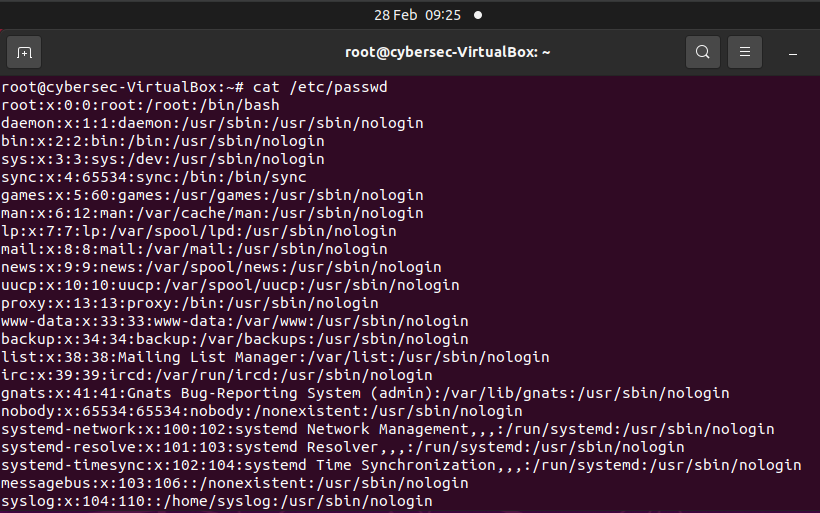
\includegraphics[width=.9\linewidth]{lab5/1}
    \caption{Making the "boys" and "girls" groups.}
    \label{fig:addgroup}
\end{figure}

\subsection{Adding users to groups}\label{subsec:adding-users-to-groups}

The new users were added to the groups mentioned above as well as the sudo group.

\begin{figure}[H]
    \centering
    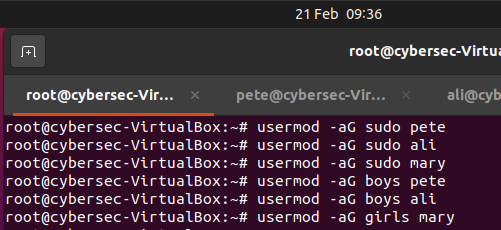
\includegraphics[width=.9\linewidth]{lab5/2}
    \caption{Adding the users to sudo and their respective groups.}
    \label{fig:addToGroup}
\end{figure}

We can verify which groups a given user is in by using the "groups" command.

\begin{figure}[H]
    \centering
    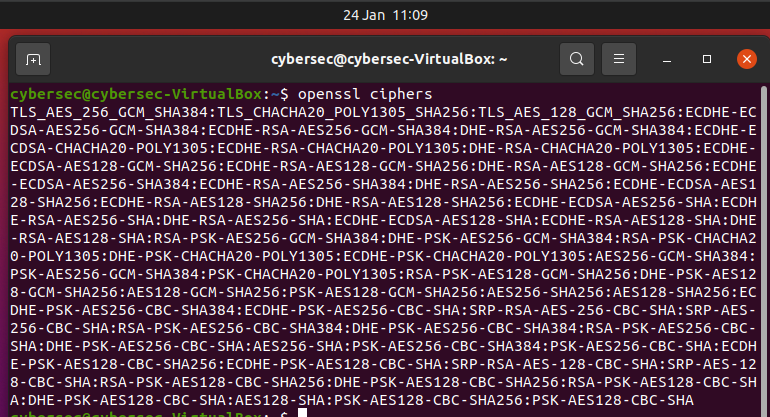
\includegraphics[width=.9\linewidth]{lab5/3}
    \caption{Verifying that the users were added to the groups.}
    \label{fig:checkGroups}
\end{figure}

This can also be checked by viewing all groups on the system via "getent groups".

\begin{figure}[H]
    \centering
    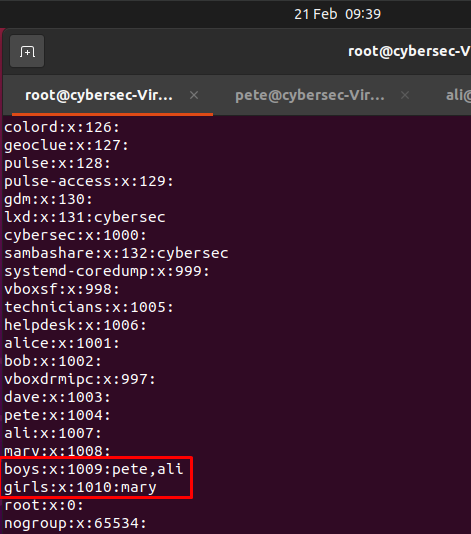
\includegraphics[width=.9\linewidth]{lab5/3b}
    \caption{Seeing all groups (Boys and Girls are highlighted).}
    \label{fig:getent}
\end{figure}

\pagebreak

\section{Using chmod and chgrp to assign permissions}\label{sec:using-chmod}
Chmod changes the permissions for a given file or directory.
It can change permissions for reading, writing and executing files for the owner of the file,
a group of users and other users\footnote{Defined as users that aren't the owner or in an
associated group with permissions.}.
I used \href{https://docs.nersc.gov/filesystems/unix-file-permissions/}{this help page}
\autocite{chmodHelp} to assist in my learning of these commands as well as access control on UNIX
systems.

\subsection{Restricting directory access}\label{subsec:chgrp}
For the purposes of testing, a directory called D1 was added to Mary's home.
This directory was associated with the girls group via chgrp, and modified with a chmod
command so that other users cannot access the directory whatsoever, but Mary and users
of the girls group can read and execute from it.

\begin{figure}[H]
    \centering
    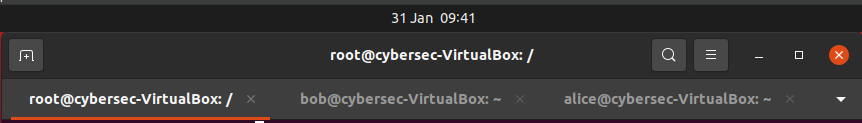
\includegraphics[width=.9\linewidth]{lab5/4}
    \caption{Creating D1 and modifying its permissions.}
    \label{fig:D1}
\end{figure}

\noindent By using the command "ls -ld", the permissions of the directory are outputted.
The returned message reveals that:
\begin{itemize}
    \item The directory owner (Mary) has \textbf{R}ead, \textbf{W}rite and e\textbf{X}ecute permissions.
    \item Group members can \textbf{R}ead and e\textbf{X}ecute.
    \item Others can only e\textbf{X}ecute.
\end{itemize}

This can be tested using Ali and Pete's accounts, which are not members of the
girls group, meaning they are "others".

\begin{figure}[H]
    \centering
    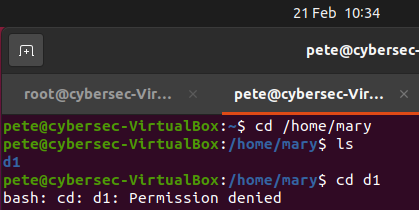
\includegraphics[width=.8\linewidth]{lab5/5}
    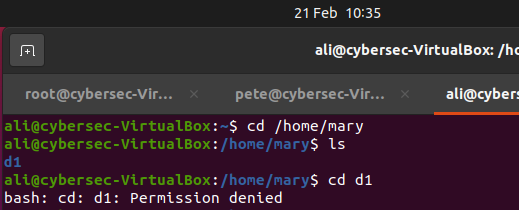
\includegraphics[width=.8\linewidth]{lab5/6}
    \caption{Attempting to access D1 as Pete and Ali.}
    \label{fig:boysD1}
\end{figure}

\begin{tcolorbox}[colback=orange!5!white,colframe=orange!75!black,title=Note]
    An issue arose here that I didn't have another user in the girls group to test access with.
    To fix this, I went back and added the existing Alice account from Lab 2 to the girls group
    with \textit{sudo usermod -aG girls alice}.
\end{tcolorbox}

Using another account in the girls group, we can test if other girls can access the directory,
which succeeds.

\begin{figure}[H]
    \centering
    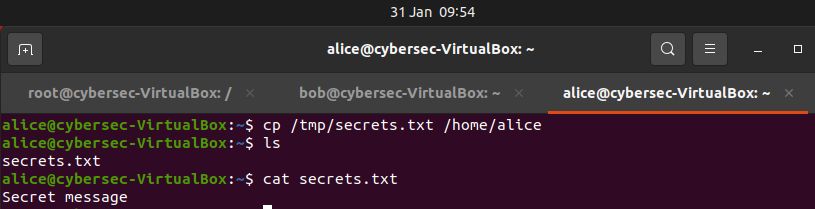
\includegraphics[width=.8\linewidth]{lab5/7}
    \caption{Successfully accessing D1 as Alice.}
    \label{fig:girlsD1}
\end{figure}

Alice is permitted to read the d1 directory and execute files
within it, but she cannot write to it, as intended.

\begin{figure}[H]
    \centering
    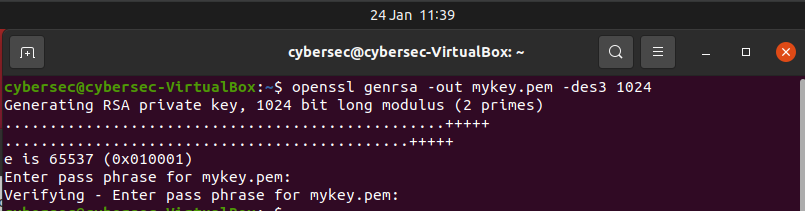
\includegraphics[width=.8\linewidth]{lab5/8}
    \caption{Failing to write to D1 as Alice.}
    \label{fig:girlsWriteD1Fail}
\end{figure}

To test this further, the permissions can then be modified\footnote{770 is "rwxrwx---", which
correlates to the file owner and members of the group having read, write and execute permissions, but other users have none.}
again to allow girls to write files, which will then allow Alice to make the file.

\begin{figure}[H]
    \centering
    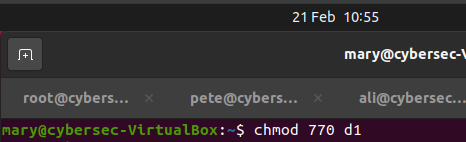
\includegraphics[width=.8\linewidth]{lab5/9}
    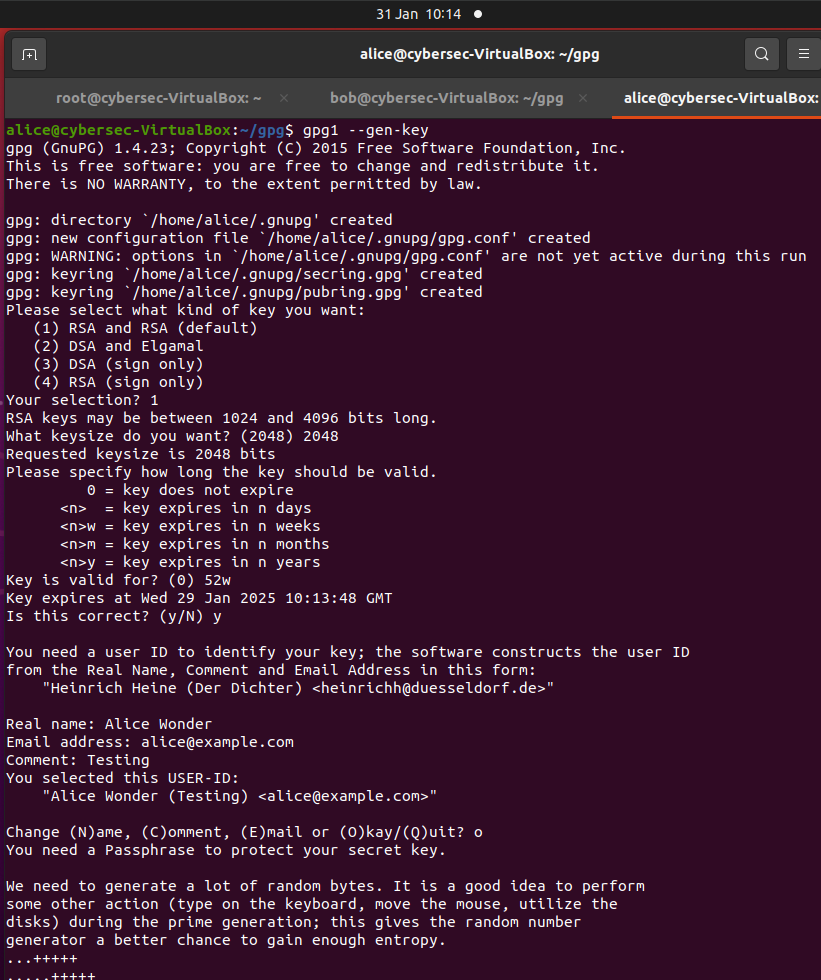
\includegraphics[width=.8\linewidth]{lab5/10}
    \caption{Modifying the permissions of D1, allowing Alice to write the file.}
    \label{fig:girlsWriteD1Success}
\end{figure}

\pagebreak

\subsection{Chgrp and chown}\label{subsec:using-chown}
\begin{tcolorbox}[colback=orange!5!white,colframe=orange!75!black,title=Note]
    I used different directory names for clarity ($BoysDirectory$ instead of $Photos$),
    but I have still demonstrated all exercises from this lab.
\end{tcolorbox}
Chown assigns a file or directory's ownership to a specific user.
For this example, we will create a directory in the shared /home folder and assign group ownership
to Boys via chgrp, and using chmod to allow all Boys all permissions, and all other users
read \& execute permissions.

\begin{figure}[H]
    \centering
    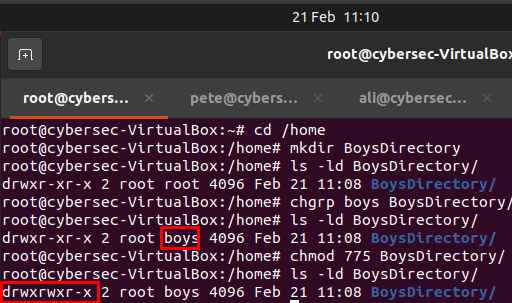
\includegraphics[width=.8\linewidth]{lab5/11}
    \caption{Making BoysDirectory and giving group ownership to Boys.}
    \label{fig:BoysDirectory}
\end{figure}

This new directory can be accessed by all users, but only written to by boys.
We can now test chown by making two subdirectories within BoysDirectory, where one will be owned
by Pete, and one by Ali.
Both users also modify the permissions of their own directories to only be accessible
by them.\footnote{700 is "rwx------", which means only the owner may read,
write and execute.}

\begin{figure}[H]
    \centering
    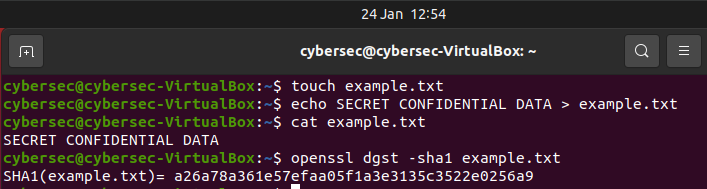
\includegraphics[width=.8\linewidth]{lab5/12}
    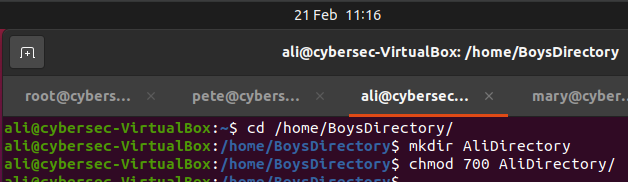
\includegraphics[width=.8\linewidth]{lab5/12b}
    \caption{Creating and modifying each user's directories and access permissions.}
    \label{fig:PeteAliDir}
\end{figure}

\begin{figure}[H]
    \centering
    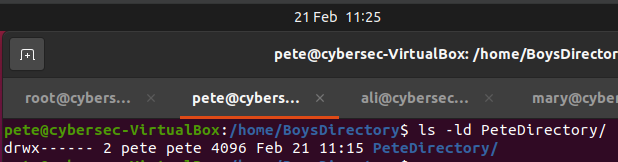
\includegraphics[width=.8\linewidth]{lab5/12c}
    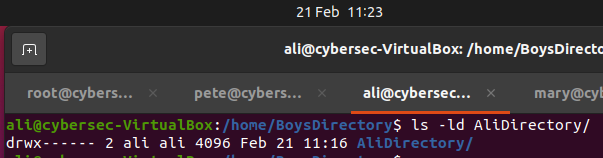
\includegraphics[width=.8\linewidth]{lab5/12d}
    \caption{Viewing the permissions of Pete and Ali's directories.}
    \label{fig:AliDirPerms}
\end{figure}

We can then prove that only the owners of the directories may access them by first accessing their
own directory, but then attempting to access the other user's directory:

\begin{figure}[H]
    \centering
    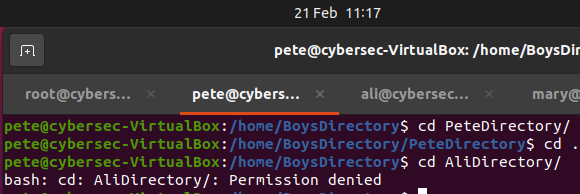
\includegraphics[width=.8\linewidth]{lab5/13}
    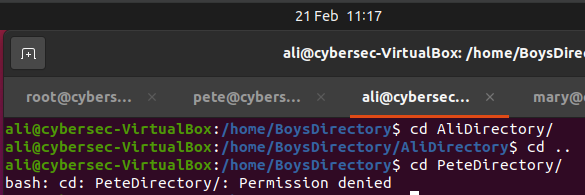
\includegraphics[width=.8\linewidth]{lab5/13b}
    \caption{Successfully accessing their own directory,
        but failing to access the other because the user isn't the owner.}
    \label{fig:PeteAliDirFail}
\end{figure}

An important distinction to be made here is that these subdirectories are owned by Pete and
Ali respectively.
They do \textbf{not} inherit the boys group ownership by default, meaning that other boys
are not considered to have group permissions over the directory until chgrp is used, as everyone who is not the owner
or in the directory's group (which is currently not set)
is considered "other" as seen in Figure \ref{fig:PeteAliDirFail}.

\begin{figure}[H]
    \centering
    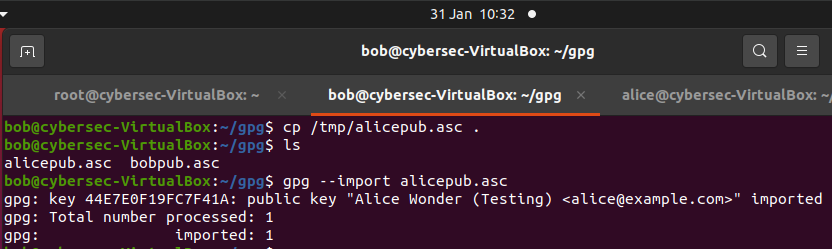
\includegraphics[width=.8\linewidth]{lab5/14}
    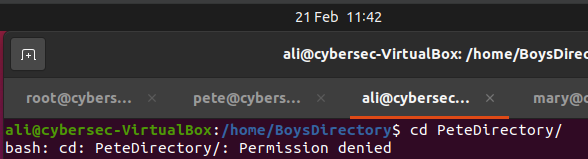
\includegraphics[width=.8\linewidth]{lab5/14b}
    \caption{Giving group RWX access to PeteDirectory, which still fails.}
    \label{fig:PeteDirFail}
\end{figure}

Ali still can't access the directory because he is not part of the "Pete" group, but he
(and any other users) would be able to use permissions given to "others".
To fix this, we can assign PeteDirectory to the Boys group.

\begin{figure}[H]
    \centering
    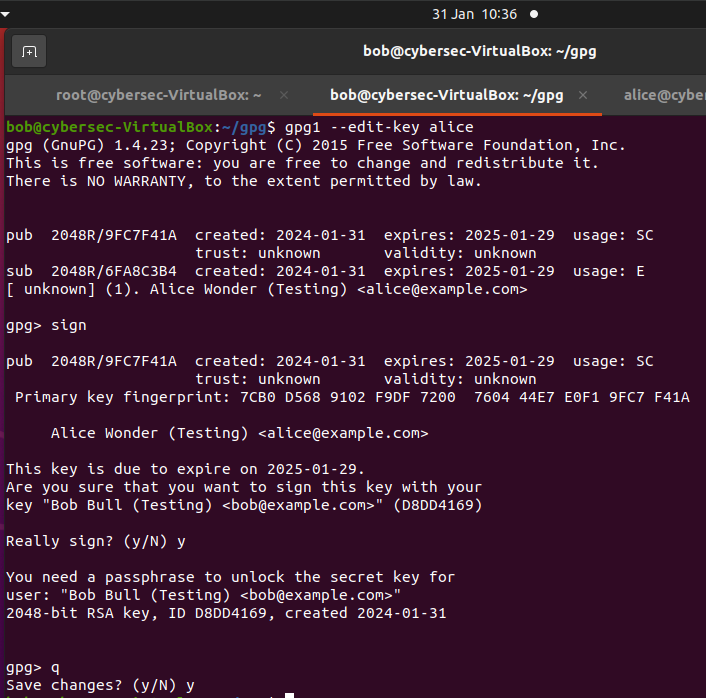
\includegraphics[width=.8\linewidth]{lab5/15}
    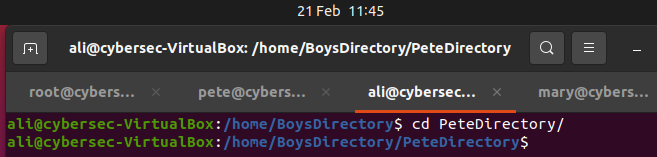
\includegraphics[width=.8\linewidth]{lab5/15b}
    \caption{Assigning PeteDirectory to boys, so Ali can now access it.}
    \label{fig:PeteDirBoys}
\end{figure}


Another option is to make Ali the directory owner, which would then give him the respective read, write
and execute permissions of Pete, and Pete would then lose these permissions due to not being the owner
anymore.
As root, we can execute "chown ali PeteDirectory" to make Ali the owner.

\begin{figure}[H]
    \centering
    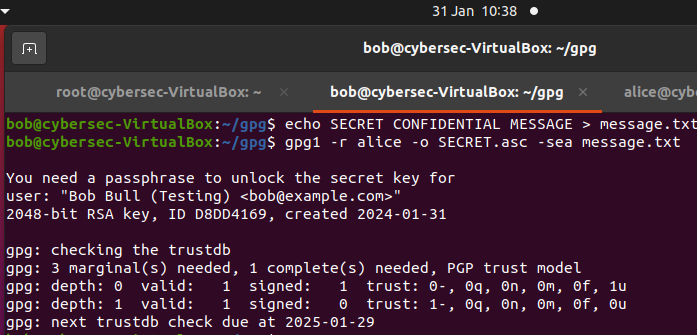
\includegraphics[width=.8\linewidth]{lab5/16}
    \caption{Making Ali the owner of PeteDirectory.}
    \label{fig:PeteDirChown}
\end{figure}

If we then remove the group permissions of Boys, instead assigning them to the "Ali" group, we can see
that Pete is definitively not the owner of this directory since he cannot access it anymore.

\begin{figure}[H]
    \centering
    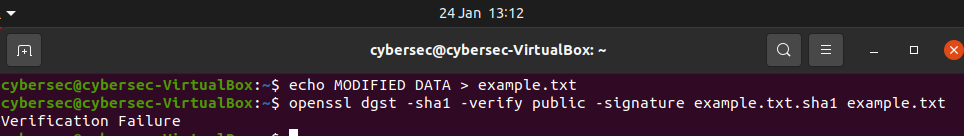
\includegraphics[width=.8\linewidth]{lab5/17}
    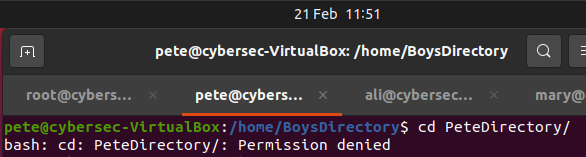
\includegraphics[width=.8\linewidth]{lab5/17b}
    \caption{Assigning PeteDirectory to the Ali group, removing Pete's access.}
    \label{fig:PeteDirAli}
\end{figure}







